\documentclass{standalone}
\usepackage{tikz}
\usetikzlibrary{patterns, positioning}


\begin{document}
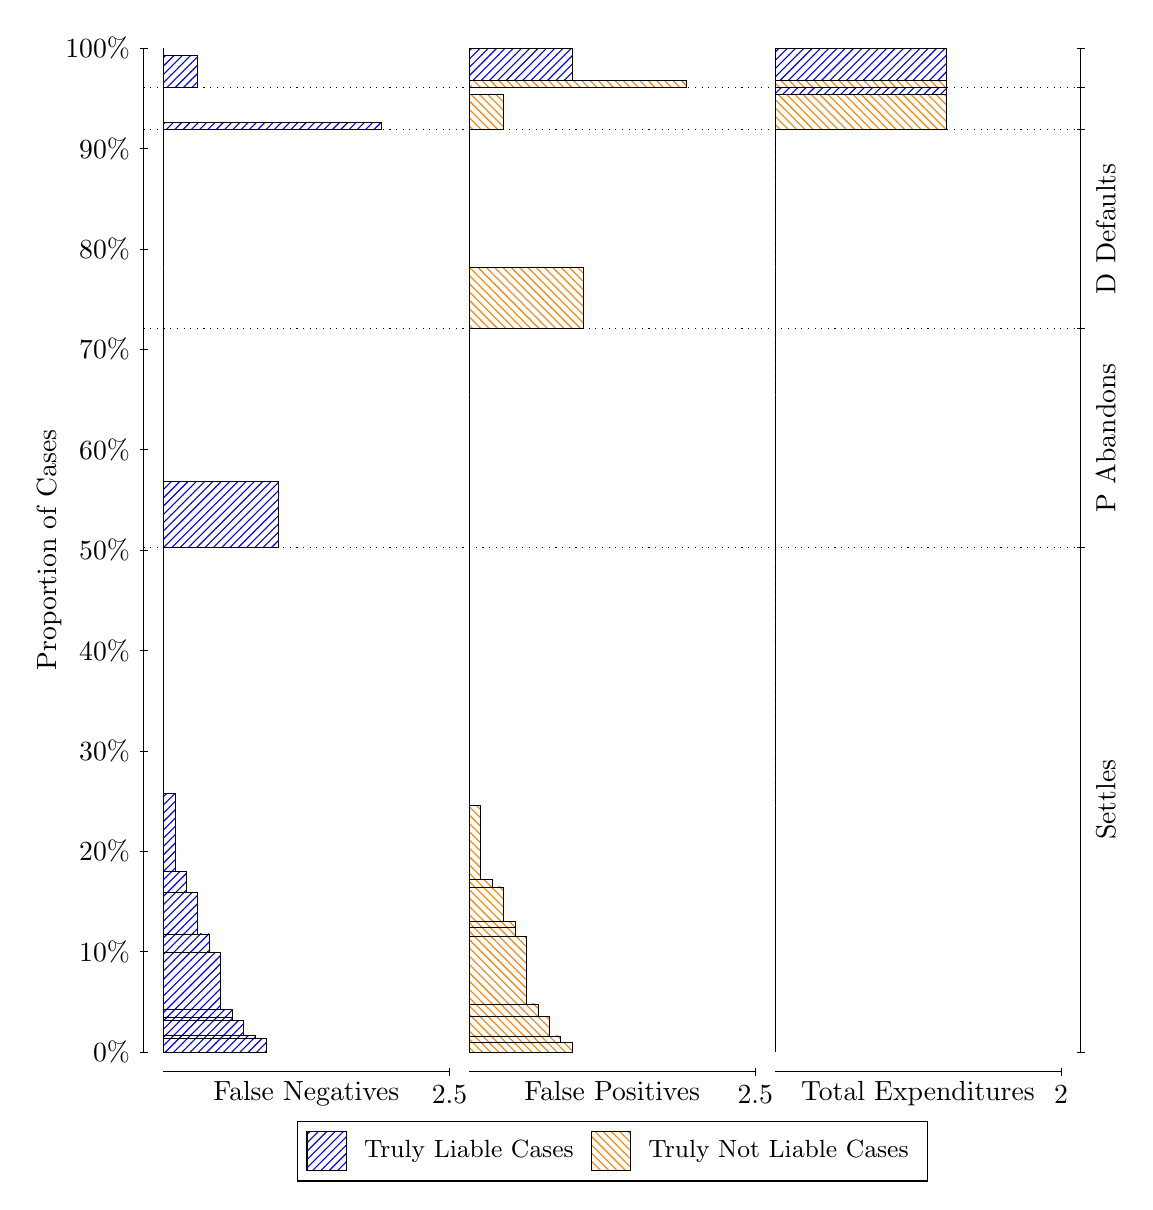
\begin{tikzpicture}
\draw[black, very thin] (1.5,1.75) -- (1.5,14.5);
\node[rotate=90, text=black, anchor=center] at (0.3, 8.125) {Proportion of Cases};
\draw[black, very thin] (1.45,1.75) -- (1.55,1.75);
\node[text=black, anchor=east] at (1.45, 1.75) {0\%};
\draw[black, very thin] (1.45,3.025) -- (1.55,3.025);
\node[text=black, anchor=east] at (1.45, 3.025) {10\%};
\draw[black, very thin] (1.45,4.3) -- (1.55,4.3);
\node[text=black, anchor=east] at (1.45, 4.3) {20\%};
\draw[black, very thin] (1.45,5.575) -- (1.55,5.575);
\node[text=black, anchor=east] at (1.45, 5.575) {30\%};
\draw[black, very thin] (1.45,6.85) -- (1.55,6.85);
\node[text=black, anchor=east] at (1.45, 6.85) {40\%};
\draw[black, very thin] (1.45,8.125) -- (1.55,8.125);
\node[text=black, anchor=east] at (1.45, 8.125) {50\%};
\draw[black, very thin] (1.45,9.4) -- (1.55,9.4);
\node[text=black, anchor=east] at (1.45, 9.4) {60\%};
\draw[black, very thin] (1.45,10.675) -- (1.55,10.675);
\node[text=black, anchor=east] at (1.45, 10.675) {70\%};
\draw[black, very thin] (1.45,11.95) -- (1.55,11.95);
\node[text=black, anchor=east] at (1.45, 11.95) {80\%};
\draw[black, very thin] (1.45,13.225) -- (1.55,13.225);
\node[text=black, anchor=east] at (1.45, 13.225) {90\%};
\draw[black, very thin] (1.45,14.5) -- (1.55,14.5);
\node[text=black, anchor=east] at (1.45, 14.5) {100\%};

\draw[black, very thin] (13.4,1.75) -- (13.4,14.5);
\draw[black, very thin] (13.35,1.75) -- (13.45,1.75);
\node[anchor=west] at (13.35, 1.75) {};
\draw[black, very thin] (13.35,8.1584) -- (13.45,8.1584);
\node[anchor=west] at (13.35, 8.1584) {};
\draw[black, very thin] (13.35,10.942) -- (13.45,10.942);
\node[anchor=west] at (13.35, 10.942) {};
\draw[black, very thin] (13.35,13.469) -- (13.45,13.469);
\node[anchor=west] at (13.35, 13.469) {};
\draw[black, very thin] (13.35,14.002) -- (13.45,14.002);
\node[anchor=west] at (13.35, 14.002) {};
\draw[black, very thin] (13.35,14.5) -- (13.45,14.5);
\node[anchor=west] at (13.35, 14.5) {};

\draw[black, very thin, pattern color=blue, pattern=north east lines] (1.75,1.75) rectangle (3.058,1.9249);
\draw[black, very thin, pattern color=blue, pattern=north east lines] (1.75,1.9249) rectangle (2.9127,1.9587);
\draw[black, very thin, pattern color=blue, pattern=north east lines] (1.75,1.9587) rectangle (2.7673,2.1544);
\draw[black, very thin, pattern color=blue, pattern=north east lines] (1.75,2.1544) rectangle (2.622,2.1949);
\draw[black, very thin, pattern color=blue, pattern=north east lines] (1.75,2.1949) rectangle (2.622,2.2904);
\draw[black, very thin, pattern color=blue, pattern=north east lines] (1.75,2.2904) rectangle (2.4767,3.0192);
\draw[black, very thin, pattern color=blue, pattern=north east lines] (1.75,3.0192) rectangle (2.3313,3.2509);
\draw[black, very thin, pattern color=blue, pattern=north east lines] (1.75,3.2509) rectangle (2.186,3.775);
\draw[black, very thin, pattern color=blue, pattern=north east lines] (1.75,3.775) rectangle (2.0407,4.042);
\draw[black, very thin, pattern color=blue, pattern=north east lines] (1.75,4.042) rectangle (1.8953,5.0306);
\draw[black, very thin, pattern color=orange, pattern=north west lines] (1.75,5.0306) rectangle (1.75,8.1584);
\draw[black, very thin, pattern color=blue, pattern=north east lines] (1.75,8.1584) rectangle (3.2033,8.9973);
\draw[black, very thin, pattern color=orange, pattern=north west lines] (1.75,8.9973) rectangle (1.75,10.942);
\draw[black, very thin, pattern color=orange, pattern=north west lines] (1.75,10.942) rectangle (1.75,11.712);
\draw[black, very thin, pattern color=blue, pattern=north east lines] (1.75,11.712) rectangle (1.75,13.469);
\draw[black, very thin, pattern color=blue, pattern=north east lines] (1.75,13.469) rectangle (4.5113,13.558);
\draw[black, very thin, pattern color=orange, pattern=north west lines] (1.75,13.558) rectangle (1.75,14.002);
\draw[black, very thin, pattern color=blue, pattern=north east lines] (1.75,14.002) rectangle (2.186,14.411);
\draw[black, very thin, pattern color=orange, pattern=north west lines] (1.75,14.411) rectangle (1.75,14.5);
\draw[black, very thin, pattern color=orange, pattern=north west lines] (5.6333,1.75) rectangle (6.9413,1.8725);
\draw[black, very thin, pattern color=orange, pattern=north west lines] (5.6333,1.8725) rectangle (6.796,1.9541);
\draw[black, very thin, pattern color=orange, pattern=north west lines] (5.6333,1.9541) rectangle (6.6507,2.2039);
\draw[black, very thin, pattern color=orange, pattern=north west lines] (5.6333,2.2039) rectangle (6.5053,2.3601);
\draw[black, very thin, pattern color=orange, pattern=north west lines] (5.6333,2.3601) rectangle (6.36,3.2149);
\draw[black, very thin, pattern color=orange, pattern=north west lines] (5.6333,3.2149) rectangle (6.2147,3.34);
\draw[black, very thin, pattern color=orange, pattern=north west lines] (5.6333,3.34) rectangle (6.2147,3.4092);
\draw[black, very thin, pattern color=orange, pattern=north west lines] (5.6333,3.4092) rectangle (6.0693,3.8477);
\draw[black, very thin, pattern color=orange, pattern=north west lines] (5.6333,3.8477) rectangle (5.924,3.9432);
\draw[black, very thin, pattern color=orange, pattern=north west lines] (5.6333,3.9432) rectangle (5.7787,4.8778);
\draw[black, very thin, pattern color=blue, pattern=north east lines] (5.6333,4.8778) rectangle (5.6333,8.1584);
\draw[black, very thin, pattern color=orange, pattern=north west lines] (5.6333,8.1584) rectangle (5.6333,10.103);
\draw[black, very thin, pattern color=blue, pattern=north east lines] (5.6333,10.103) rectangle (5.6333,10.942);
\draw[black, very thin, pattern color=orange, pattern=north west lines] (5.6333,10.942) rectangle (7.0867,11.712);
\draw[black, very thin, pattern color=blue, pattern=north east lines] (5.6333,11.712) rectangle (5.6333,13.469);
\draw[black, very thin, pattern color=orange, pattern=north west lines] (5.6333,13.469) rectangle (6.0693,13.913);
\draw[black, very thin, pattern color=blue, pattern=north east lines] (5.6333,13.913) rectangle (5.6333,14.002);
\draw[black, very thin, pattern color=orange, pattern=north west lines] (5.6333,14.002) rectangle (8.3947,14.09);
\draw[black, very thin, pattern color=blue, pattern=north east lines] (5.6333,14.09) rectangle (6.9413,14.5);
\draw[black, very thin, pattern color=orange, pattern=north west lines] (9.5167,1.75) rectangle (9.5167,4.8778);
\draw[black, very thin, pattern color=blue, pattern=north east lines] (9.5167,4.8778) rectangle (9.5167,8.1584);
\draw[black, very thin, pattern color=orange, pattern=north west lines] (9.5167,8.1584) rectangle (9.5167,10.103);
\draw[black, very thin, pattern color=blue, pattern=north east lines] (9.5167,10.103) rectangle (9.5167,10.942);
\draw[black, very thin, pattern color=orange, pattern=north west lines] (9.5167,10.942) rectangle (9.5167,11.712);
\draw[black, very thin, pattern color=blue, pattern=north east lines] (9.5167,11.712) rectangle (9.5167,13.469);
\draw[black, very thin, pattern color=orange, pattern=north west lines] (9.5167,13.469) rectangle (11.697,13.913);
\draw[black, very thin, pattern color=blue, pattern=north east lines] (9.5167,13.913) rectangle (11.697,14.002);
\draw[black, very thin, pattern color=orange, pattern=north west lines] (9.5167,14.002) rectangle (11.697,14.09);
\draw[black, very thin, pattern color=blue, pattern=north east lines] (9.5167,14.09) rectangle (11.697,14.5);
\draw[black, dotted] (1.5,8.1584) -- (13.4,8.1584);
\draw[black, dotted] (1.5,10.942) -- (13.4,10.942);
\draw[black, dotted] (1.5,13.469) -- (13.4,13.469);
\draw[black, dotted] (1.5,14.002) -- (13.4,14.002);
\draw[black, very thin] (1.75,1.5) -- (5.3833,1.5);
\node[text=black, anchor=north] at (3.5667, 1.5) {False Negatives};
\draw[black, very thin] (5.3833,1.45) -- (5.3833,1.55);
\node[text=black, anchor=north] at (5.3833, 1.45) {2.5};

\draw[black, very thin] (5.6333,1.5) -- (9.2667,1.5);
\node[text=black, anchor=north] at (7.45, 1.5) {False Positives};
\draw[black, very thin] (9.2667,1.45) -- (9.2667,1.55);
\node[text=black, anchor=north] at (9.2667, 1.45) {2.5};

\draw[black, very thin] (9.5167,1.5) -- (13.15,1.5);
\node[text=black, anchor=north] at (11.333, 1.5) {Total Expenditures};
\draw[black, very thin] (13.15,1.45) -- (13.15,1.55);
\node[text=black, anchor=north] at (13.15, 1.45) {2};

\node[text=black, centered, rotate=90] at (13.72, 4.9542) {Settles};
\node[text=black, centered, rotate=90] at (13.72, 9.5501) {P Abandons};
\node[text=black, centered, rotate=90] at (13.72, 12.205) {D Defaults};



\draw (7.449999999999999,1.5) node[draw=none] (baseCoordinate) {};
\begin{scope}[align=center]
        \matrix[scale=0.5, draw=black, below=0.5cm of baseCoordinate, nodes={draw}, column sep=0.1cm]{
            \node[rectangle, draw, minimum width=0.5cm, minimum height=0.5cm, pattern color=blue, pattern=north east lines] {}; &
            \node[draw=none, font=\small, text=black] (B) {Truly Liable Cases}; &
            \node[rectangle, draw, minimum width=0.5cm, minimum height=0.5cm, pattern color=orange, pattern=north west lines] {}; &
            \node[draw=none, font=\small, text=black] (B) {Truly Not Liable Cases}; \\
            };
\end{scope}

\end{tikzpicture}
\end{document}